\subsection{问题背景}
“穿越沙漠”是一个以资源受限条件下路径规划与决策优化为核心的策略类游戏。
%
玩家需要在给定地图上，从起点出发，穿越沙漠并最终到达终点。
%
游戏过程中，玩家必须合理安排每日行动、购买和消耗水与食物，
%
并结合天气变化、村庄补给和矿山挖矿等机制制定最优策略，以保证在规定期限内完成穿越任务，
%
同时尽可能保留更多资金。具体规则如下：

\begin{figure}[H]
    \centering
    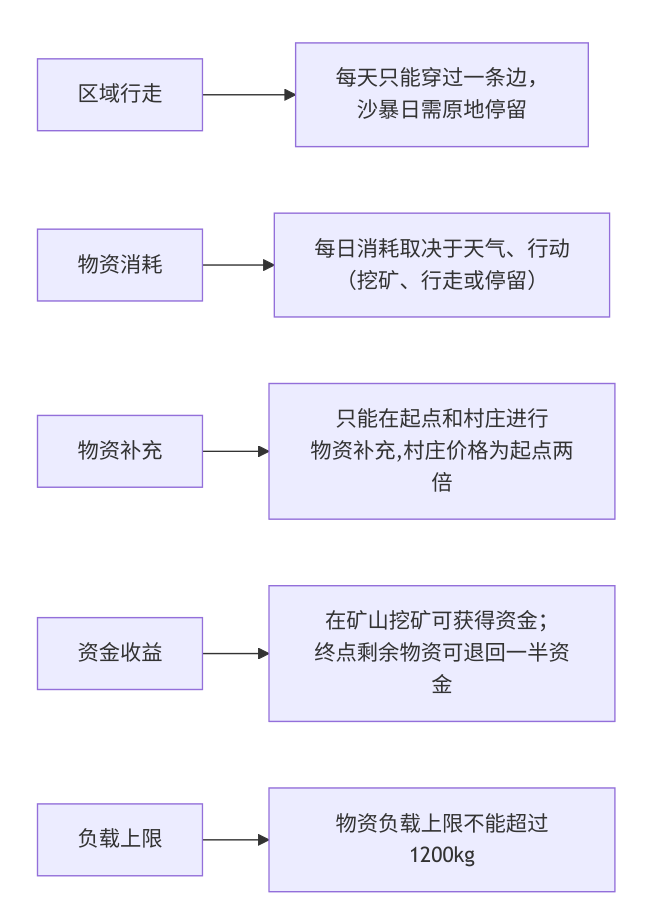
\includegraphics[width=0.7\textwidth]{C2020b/figure/问题背景.png}
    \caption{问题背景}
\end{figure}

此外，在多名玩家的情况下，还存在同行物资消耗翻倍、多人同时挖矿收益压缩等规则。

\subsection{需解决的问题}

根据题目设定，需要针对不同信息条件和参与人数建立相应模型，为玩家制定最优或近优策略，
%
使其在成功到达终点的前提下剩余资金尽可能多。具体需要解决如下问题：

\begin{itemize}
    \item 问题一：单人、天气完全已知情形。
        假设仅有一名玩家参与游戏，且在整个游戏周期内每天的天气状况均已提前知道。
        需要在已知天气序列、地图结构、资源价格、负重上限和截止日期的前提下，
        确定玩家每天的最优行动方案，包括是否移动、是否停留、是否前往村庄补给、是否前往矿山挖矿，
        以及初始阶段应购入多少水和食物，并对附件中的前两关进行求解。
    \item 问题二：单人、天气部分未知情形。
        假设仍只有一名玩家，但玩家仅知道当天的天气，而无法提前获知未来天气状况，
        只能根据当前状态决定当天行动。此时需要建立适用于随机天气环境下的动态决策模型，
        使玩家能够依据当前位置、剩余资源、剩余资金和剩余时间实时调整策略，
        并对附件中的第三关和第四关进行讨论。
    \item 问题三第一问：多人、天气已知情形。
        当有多名玩家同时从起点出发，且天气信息完全已知时，每位玩家的行动方案需在第1天确定后不再改变。
        由于多人同行、同矿和同村补给会引起资源消耗、收益和价格变化，因此需要建立多人协同优化模型，
        确定各玩家应采取的路径与分工策略，并对附件中的第五关进行具体分析。
    \item 问题三第二问：多人、天气部分未知情形。 
        假设多名玩家仅知道当天的天气状况，并且从第2天起，
        所有玩家在每天结束后都可以获知其他玩家当日的行动方案及剩余资源情况，然后再决定下一天的行动。
        这一情形下，玩家之间既存在竞争，也存在一定的信息互动与协同关系。需要建立适用于动态博弈环境的决策模型，
        研究一般情况下玩家应采取的策略，并对附件中的第六关进行讨论。
\end{itemize}